\section{Background}

A barcode is an optical machine-readable representation of data relating to the object
to which it is attached. Originally barcodes systematically represented data by varying the
widths and spacings of parallel lines, and may be referred to as linear or one-dimensional
(1D). Later two-dimensional (2D) codes were developed, using rectangles, dots, hexagons
and other geometric patterns in two dimensions, usually called barcodes although they do
not use bars as such. Barcodes originally were scanned by special optical scanners called
barcode readers. Later applications software became available for devices that could read
images, such as smartphones with cameras.


Nowadays the most applied barcode is QR code, integrated in applications like
Wechat, Paypal, Alipay etc. QR code (abbreviated from Quick Response Code) is the
trademark for a type of matrix barcode (or two-dimensional barcode) first designed for the
automotive industry in Japan. A QR code uses four standardized encoding modes
(numeric, alphanumeric, byte/binary, and kanji) to efficiently store data; extensions may
also be used.


The QR Code system became popular outside the automotive industry due
to its fast readability and greater storage capacity compared to standard UPC barcodes.
Applications include product tracking, item identification, time tracking, document
management, and general marketing.
A QR code consists of black modules (square dots)
arranged in a square grid on a white background, which can be read by an imaging
device (such as a camera, scanner, etc.) and processed using Reed–Solomon error
correction until the image can be appropriately interpreted. The required data are then
extracted from patterns that are present in both horizontal and vertical components of the
image.

In this lab, we will use the skeleton code based on ZXing ("zebra crossing"), an open-source, multi-format 1D/2D barcode image processing library implemented in Java, with ports to other languages, and build an mobile app that can encode and decode barcodes.

In this report, we first introduce how to setup the environment, then we will walk through the codes and finally demonstrates the mobile app on a real machine.

\section{Environment Setup}


The environment of this experiment is listed as follows. I could not run Android Studio on my computer and used Intellij IDEA as an alternative.

\begin{itemize}
  \item Development Envrionment OS: macOS 11.2
  \item IDE: Intellij IDEA Ultimate 2020.2
  \item Android SDK 21
\end{itemize}

We also modified the \texttt{app/gradle.build} file as follows in order to sync our IDE with the project.

\begin{lstlisting}
apply plugin: 'com.android.application'

android {
    compileSdkVersion 21 
    // should be consistent with buildToolsVersion/targetSdkVersion
    buildToolsVersion "21.0.2" // <-- This is changed

    defaultConfig {
        applicationId "edu.sjtu.zhusy54.qrcode"
        minSdkVersion 14
        targetSdkVersion 21
        versionCode 1
        versionName "1.0"
    }
    buildTypes {
        release {
            minifyEnabled false
            proguardFiles getDefaultProguardFile('proguard-android.txt'), \
            'proguard-rules.pro'
        }
    }
    lintOptions {
        abortOnError false
    }
}

dependencies {
    compile fileTree(dir: 'libs', include: ['*.jar'])
    testCompile 'junit:junit:4.12'
    compile 'com.android.support:appcompat-v7:21.0.2' // <-- This is changed
}
    
\end{lstlisting}

Then the gradle can generate the build/assemble scripts for the application project and we can continue with the experiment.

\section{Implementation Details}

\subsection{\texttt{MainActivity}}

Initially, the \texttt{onCreate} phase of the \texttt{MainActivity} class will set up two listeners for the encoder and decoder button, so that the corresponding view can be activated when user clicks the button. 

This class also implements a method called \texttt{onActivityResult}, which enables the \texttt{TestDecoder} to pop an alert message to the user indicating the decoding result after a QR code is scanned.

\subsection{\texttt{TestDecoder}}

The key function of a decoder is to open the camera, looking for a QRcode and returns it to the \texttt{MainActivity} as soon as a QRcode is detected. They are mainly implemented in \texttt{surfaceCreated} method. The code for this method is listed as follows.

\begin{lstlisting}[language=java]
public void surfaceCreated(SurfaceHolder holder)
{
    mCamera = Camera.open();// open camera
    try
    {
        Log.i("TAG", "SurfaceHolder.Callback:surface Created");
        mCamera.setPreviewDisplay(mSurfaceHolder);
        //set the surface to be used for live preview
    }catch (Exception ex)
    {
        if(null != mCamera)
        {
            mCamera.release();
            mCamera = null;
        }
        Log.i("TAG"+"initCamera", ex.getMessage());
    }
    mCamera.setPreviewCallback(new Camera.PreviewCallback(){

        @Override
        public void onPreviewFrame(byte[] data, Camera camera) {
            int previewWidth = camera.getParameters().getPreviewSize().width;
            int previewHeight = camera.getParameters().getPreviewSize().height;

            PlanarYUVLuminanceSource source = new PlanarYUVLuminanceSource(
                    data, previewWidth, previewHeight, 0, 0, previewWidth,
                    previewHeight, false);
            BinaryBitmap bitmap = new BinaryBitmap(new HybridBinarizer(source));

            Reader reader = new QRCodeReader();
            try {

                Result result = reader.decode(bitmap);
                String text = result.getText();

                Intent intent = new Intent();
                Bundle bundle = new Bundle();
                bundle.putString("result", result.toString());
                intent.putExtras(bundle);
                setResult(RESULT_OK, intent);
                finish();
            } catch (Exception e) {
                e.printStackTrace();
            }
        }
    });
\end{lstlisting}

Note that a \texttt{QRCodeReader} instance is created. This is a module provided by the \texttt{zxing} package, which can detect and decode QR Codes in an image. We see that once a decoding result is obtained in the \texttt{result}. A \texttt{setResult} method will be called and pass that result to \texttt{MainActivity}. The scanned result will be alerted to the user by \texttt{MainActivity}.

With a few extra configuring codes that set up the camera, we can finish implementing the QRcode decoder.


\subsection{\texttt{TestEncoder}}

The implementation of the encoding function is basically written in the listener of the \texttt{Generate} button, listed as follows.

\begin{lstlisting}[language=java]
genBtn.setOnClickListener(new View.OnClickListener() {
    @Override
    public void onClick(View v) {
        try {
            String contentString = textContent.getText().toString();
            if (!contentString.equals("")) {
                BitMatrix matrix = new MultiFormatWriter().encode(contentString,
                        BarcodeFormat.QR_CODE, 300, 300);
                int width = matrix.getWidth();
                int height = matrix.getHeight();
                int[] pixels = new int[width * height];

                for (int y = 0; y < height; y++) {
                    for (int x = 0; x < width; x++) {
                        if (matrix.get(x, y)) {
                            pixels[y * width + x] = Color.BLACK;
                        }
                    }
                }
                Bitmap bitmap = Bitmap.createBitmap(width, height,
                        Bitmap.Config.ARGB_8888);
                bitmap.setPixels(pixels, 0, width, 0, 0, width, height);
                ImageView image1 = new ImageView(TestEncoder.this);
                image1.setImageBitmap(bitmap);
                new AlertDialog.Builder(TestEncoder.this)
                        .setTitle("QR Code")
                        .setIcon(android.R.drawable.ic_dialog_info)
                        .setView(image1)
                        .setPositiveButton("Confirm", new DialogInterface.OnClickListener(){
                            @Override
                            public void onClick(DialogInterface dialog, int which) {
                                dialog.dismiss();
                            }
                        })
                        .show();
            } else {
                Toast.makeText(TestEncoder.this, "Text can not be empty", Toast.LENGTH_SHORT).show();
            }

        } catch (WriterException e) {
            e.printStackTrace();
        }
    }
}
\end{lstlisting}


The key module this function uses is \texttt{MultiFormatWriter}, which is a factory class implemented in \texttt{Zxing} which finds the appropriate Writer subclass for the BarcodeFormat requested and encodes the barcode with the supplied contents. The generated QRcode will be written in to a \texttt{matrix} object. Then our code will convert this matrix into an image and put it on the alert window.

Above, along with some other codes that deal with side cases or set up the environment, the encoding function is implemented.

\section{Demonstration}

The Encoder function is shown in Figure \ref{fig:encode} and the Decoder function is shown in Figure \ref{fig:decode}

\begin{figure}[hb]
  \begin{center}
  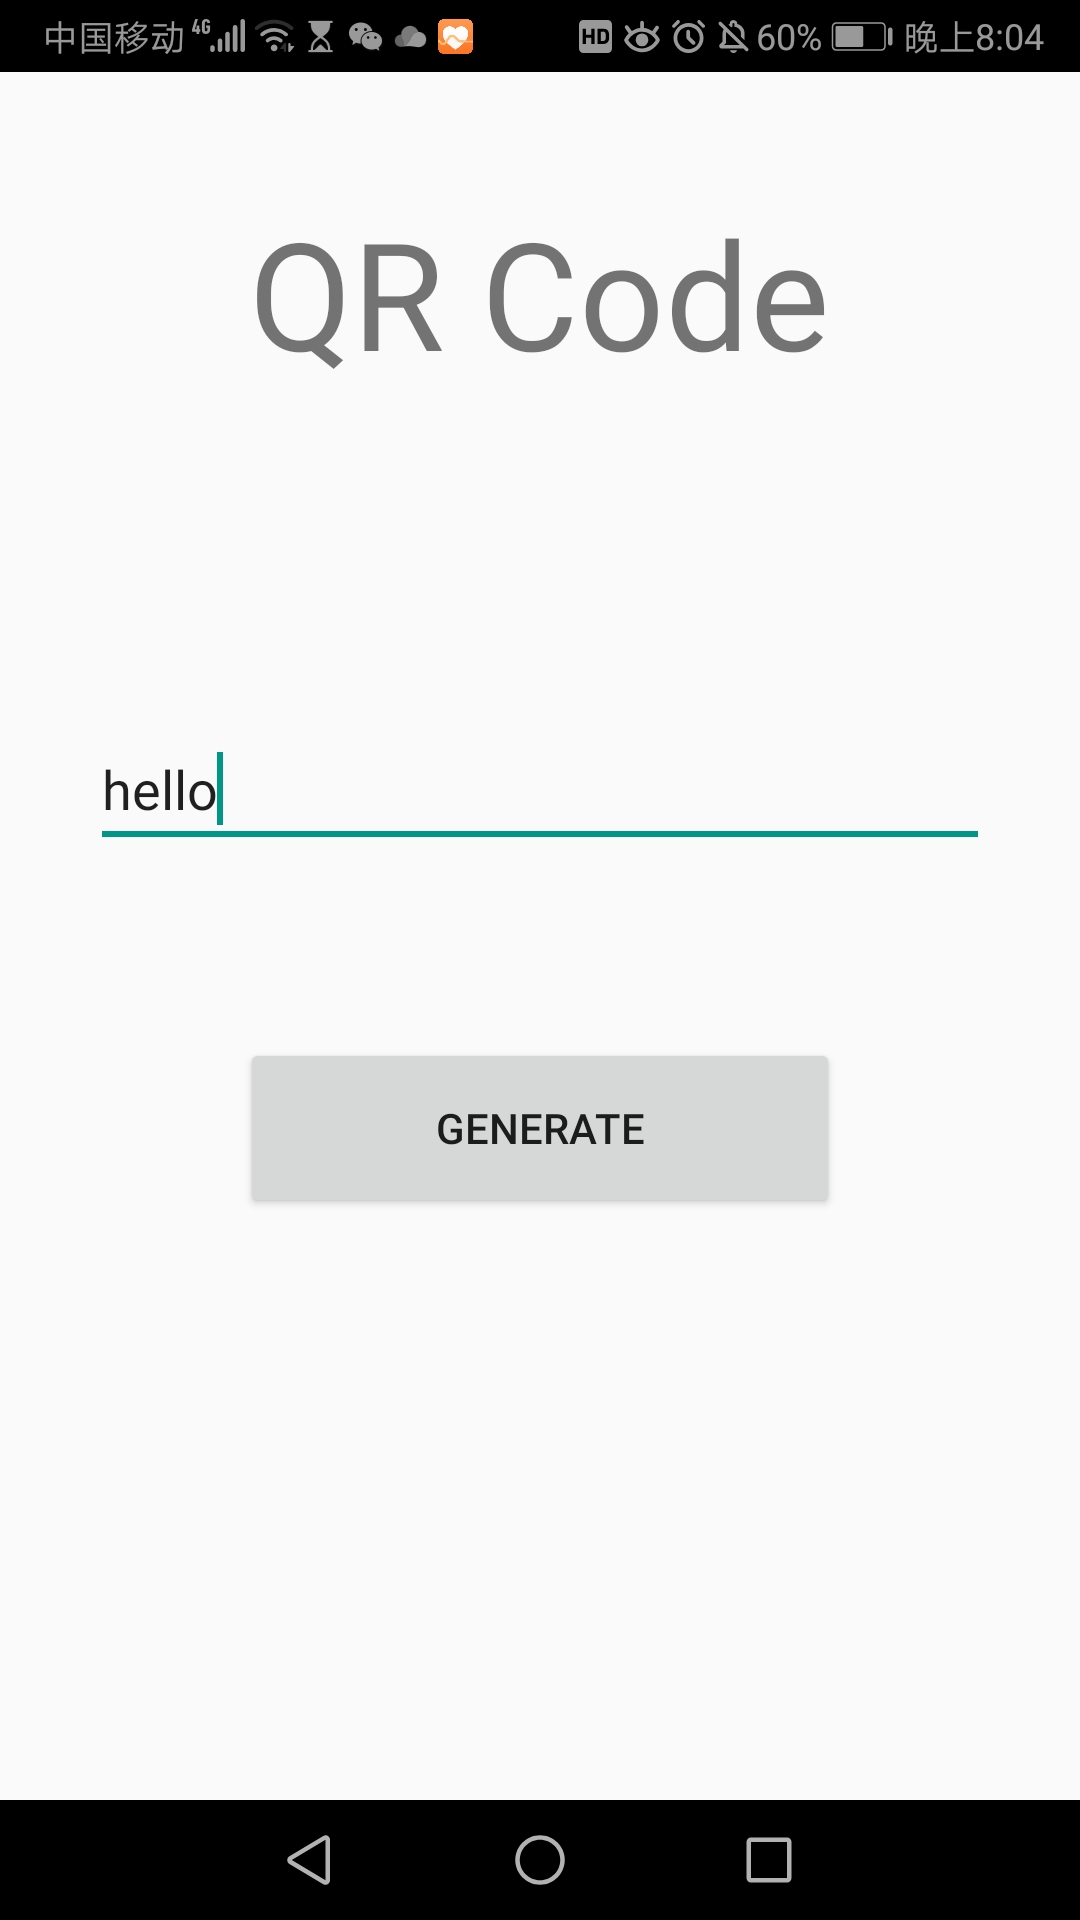
\includegraphics[width=5cm]{img/encode1.jpeg}
  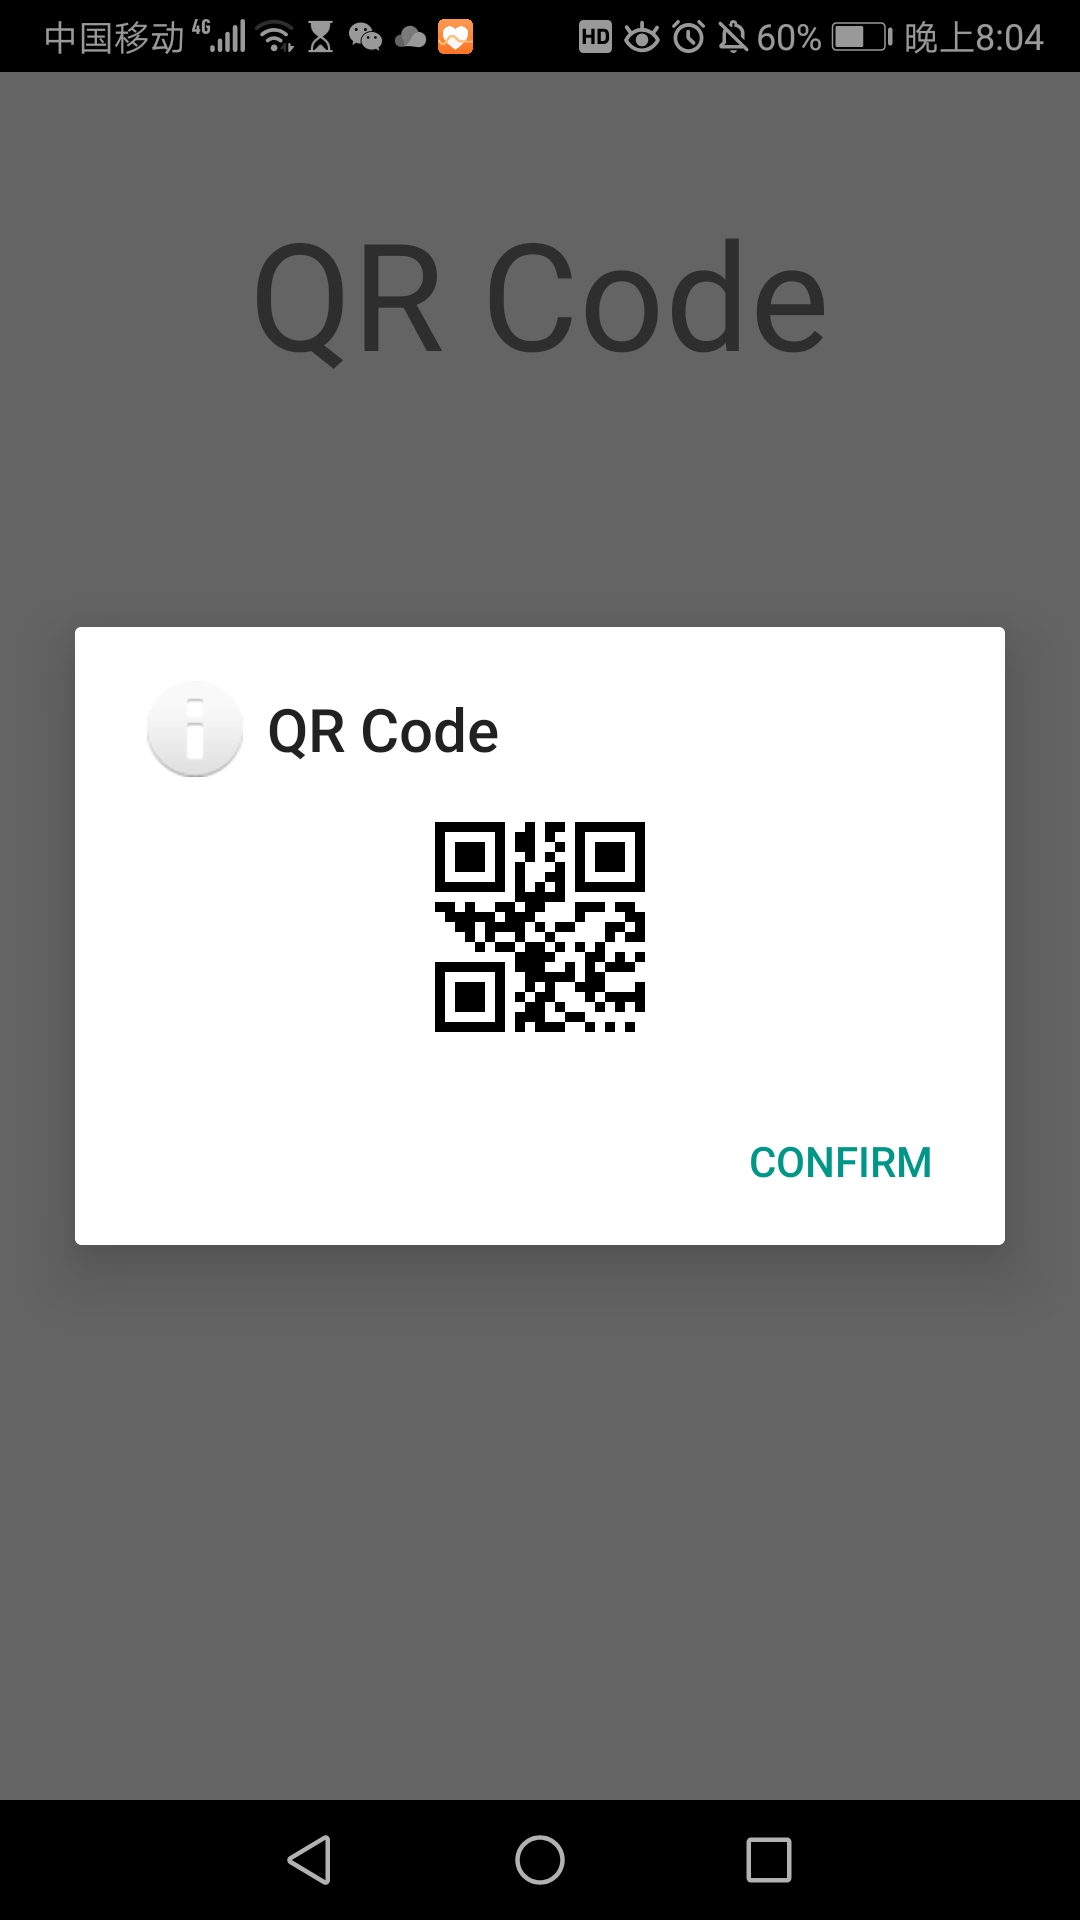
\includegraphics[width=5cm]{img/encode2.jpeg}
  \caption{Encoder Output}
  \label{fig:encode}
  \end{center}
\end{figure}

\begin{figure}[hb]
\begin{center}
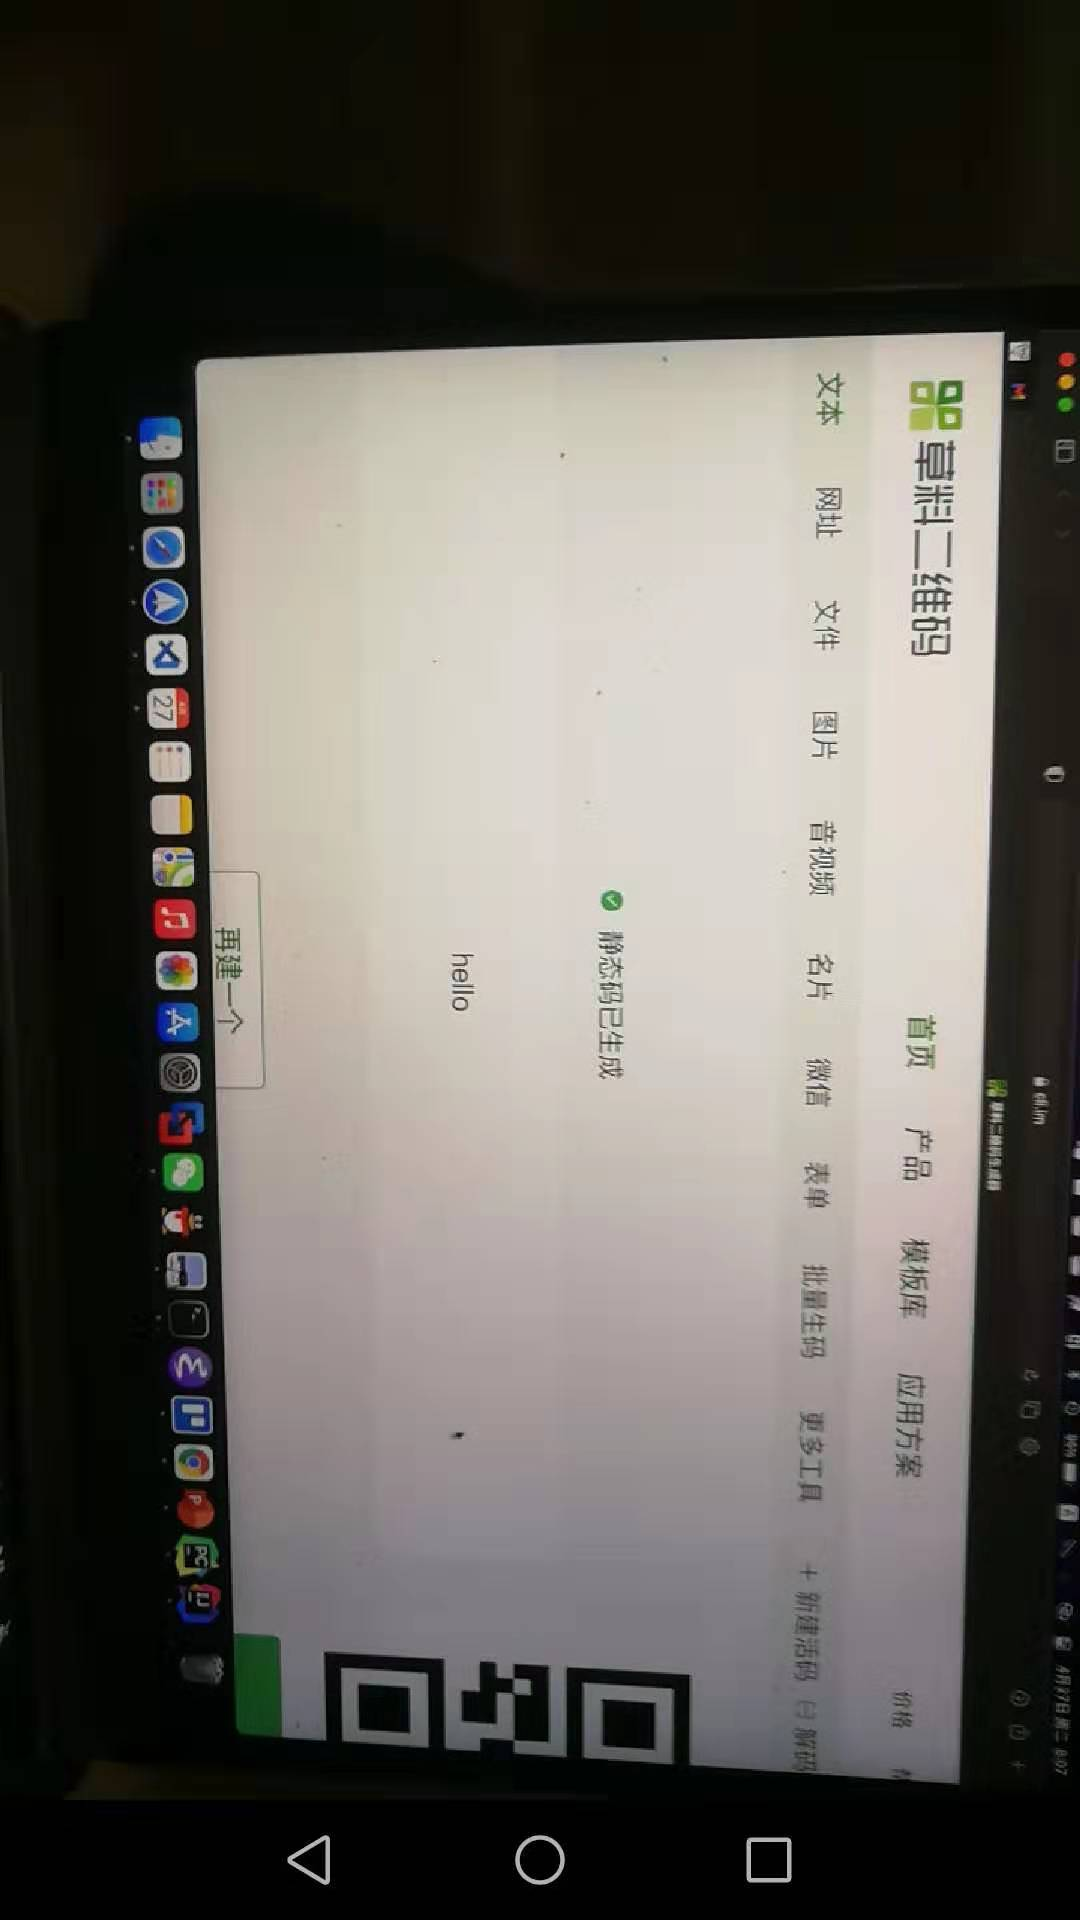
\includegraphics[width=5cm]{img/decode1.jpeg}
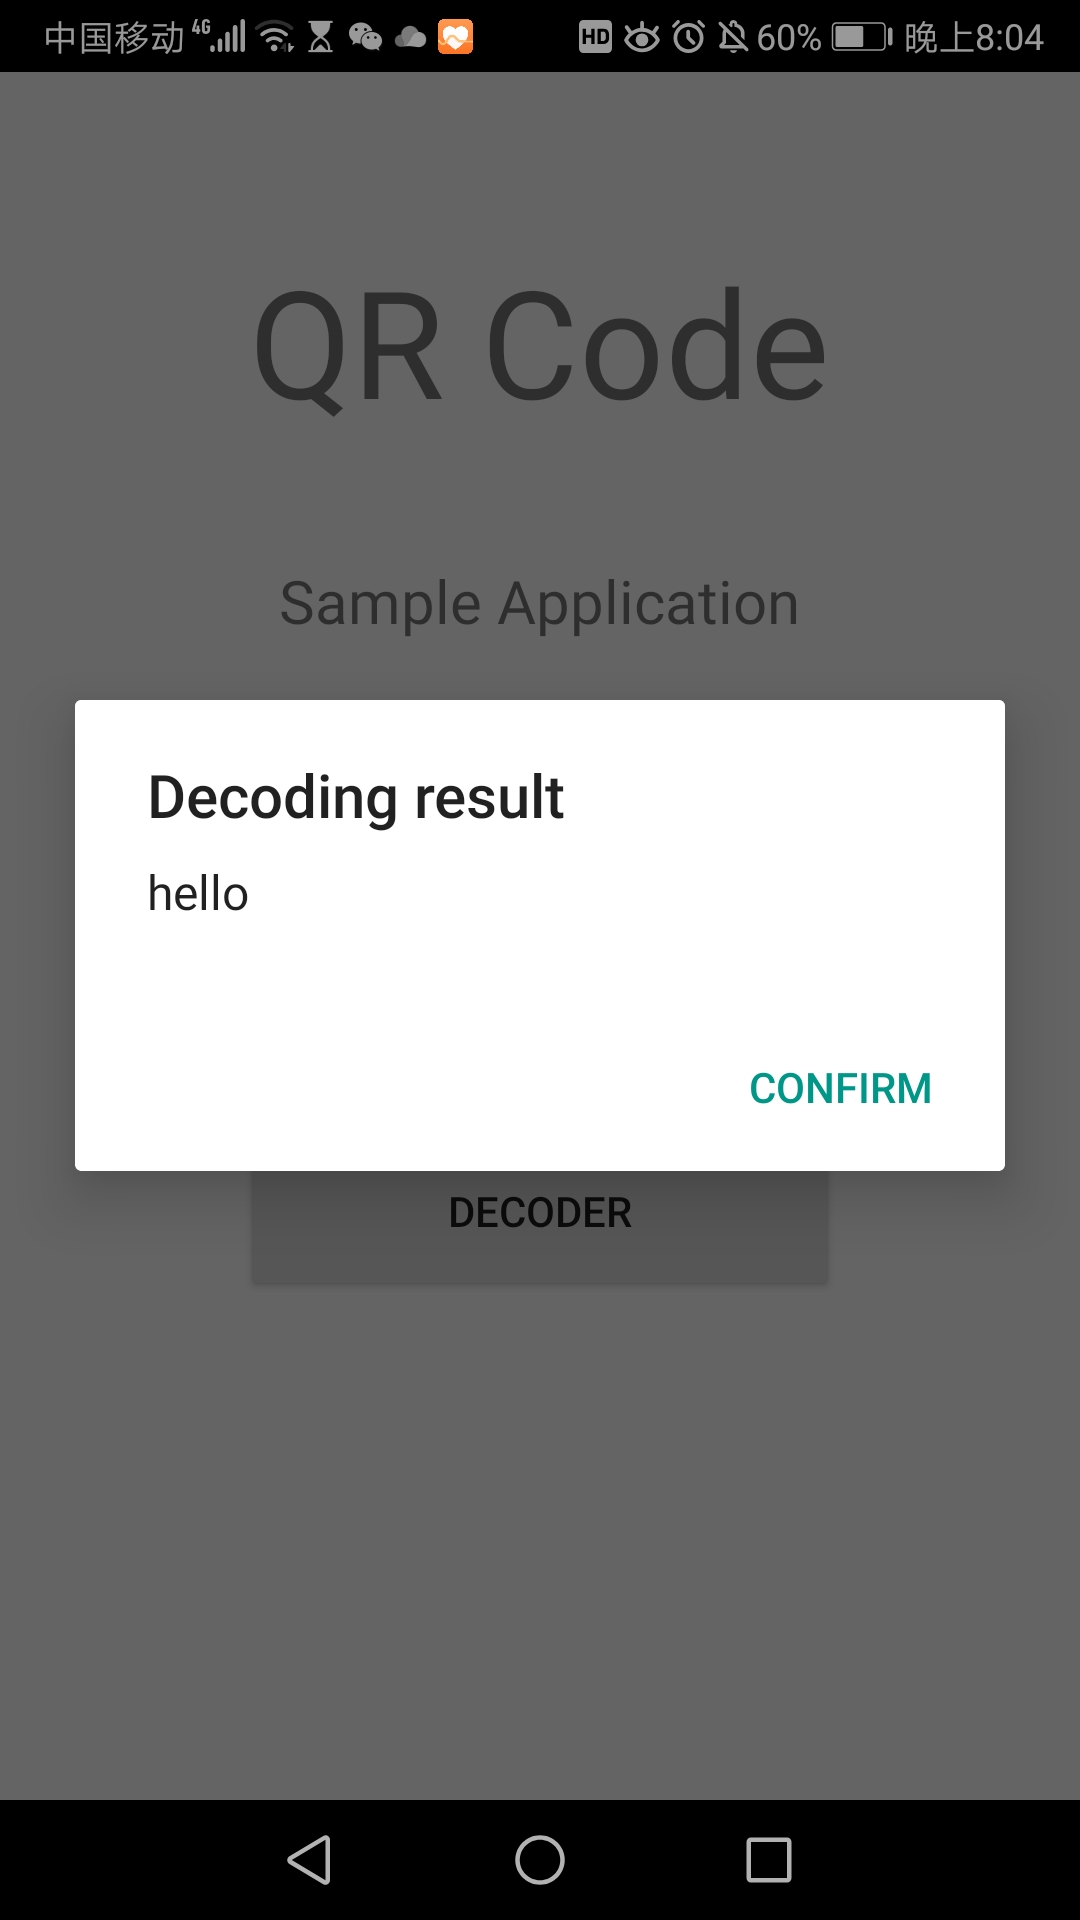
\includegraphics[width=5cm]{img/decode2.jpeg}
\caption{Decoder Output for a ``Hello'' string}
\label{fig:decode}
\end{center}
\end{figure}